\documentclass[tikz,border=2pt]{standalone}
\usepackage{amsmath}
\usepackage{pgfplots}
\pgfplotsset{compat=1.18}
\usetikzlibrary{arrows.meta}
\begin{document}
% Two-type signalling game: in the candidate separating profile (H sends m = 1, L sends m = 0) the
% receiver accepts after m = 1 (sender gets 2) and rejects after m = 0 (sender gets 0).
% Incentive constraints: H: 2 - c_H >= 0 iff c_H <= 2, L: 0 >= 2 - c_L iff c_L >= 2. The shaded set
% is where the separating PBE exists; (1, 3) is inside, (1, 1.5) is outside because L would mimic
% (2 - 1.5 = 0.5 > 0).
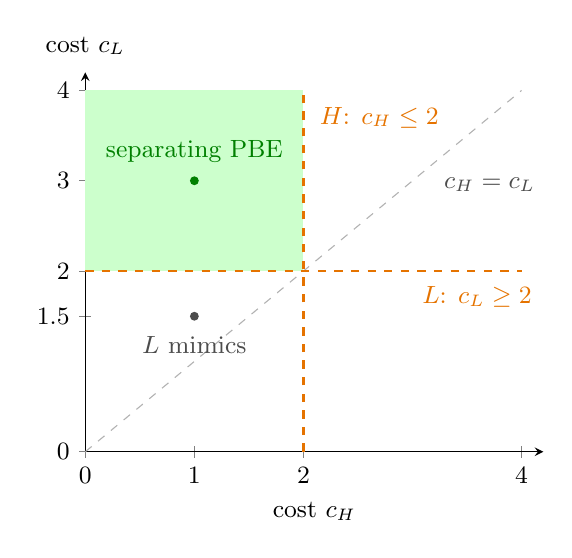
\begin{tikzpicture}[font=\small, >={Latex[length=2mm]}]
  \begin{axis}[
    axis lines=left, xmin=0, xmax=4.2, ymin=0, ymax=4.2,
    xtick={0,1,2,4}, ytick={0,1.5,2,3,4},
    xticklabels={$0$,$1$,$2$,$4$}, yticklabels={$0$,$1.5$,$2$,$3$,$4$},
    xlabel={cost $c_H$}, ylabel={cost $c_L$},
    ylabel style={rotate=-90, anchor=south, at={(axis description cs:0,1.02)}},
    width=7.4cm, height=6.4cm, clip=false]
    \addplot[fill=green!20, draw=none] coordinates {(0,2) (2,2) (2,4) (0,4)} -- cycle;
    \addplot[gray!60, thin, dashed] coordinates {(0,0) (4,4)};
    \addplot[orange!90!black, thick, dashed] coordinates {(2,0) (2,4)};
    \addplot[orange!90!black, thick, dashed] coordinates {(0,2) (4,2)};
    \fill[green!50!black] (axis cs:1,3) circle (1.6pt);
    \fill[gray!60!black] (axis cs:1,1.5) circle (1.6pt);
    \node[green!50!black, anchor=south] at (axis cs:1,3.1) {separating PBE};
    \node[gray!60!black, anchor=north] at (axis cs:1,1.38) {$L$ mimics};
    \node[orange!90!black, anchor=west] at (axis cs:2.06,3.7) {$H$: $c_H\le2$};
    \node[orange!90!black, anchor=north west] at (axis cs:3,1.94) {$L$: $c_L\ge2$};
    \node[gray!60!black, anchor=west] at (axis cs:3.2,2.96) {$c_H=c_L$};
  \end{axis}
\end{tikzpicture}
\end{document}
